\documentclass[letterpaper]{article} % DO NOT CHANGE THIS
\usepackage[submission]{aaai2027}  % DO NOT CHANGE THIS
% The serif, sans-serif, and monospaced fonts are loaded automatically by
% aaai2027.sty (newtxtext, helvet, courier). DO NOT add \usepackage{times},
% \usepackage{helvet}, \usepackage{courier}, or any other font package.
\usepackage[hyphens]{url}  % DO NOT CHANGE THIS
\usepackage{graphicx} % DO NOT CHANGE THIS
\urlstyle{rm} % DO NOT CHANGE THIS
\def\UrlFont{\rm}  % DO NOT CHANGE THIS
\usepackage{natbib}  % DO NOT CHANGE THIS AND DO NOT ADD ANY OPTIONS TO IT
\usepackage{caption} % DO NOT CHANGE THIS AND DO NOT ADD ANY OPTIONS TO IT
\frenchspacing  % DO NOT CHANGE THIS
%
% These are recommended to typeset algorithms but not required. See the subsubsection on algorithms. Remove them if you don't have algorithms in your paper.
\usepackage{algorithm}
\usepackage{algorithmic}
\usepackage{comment}
\usepackage{amsmath,amssymb,amsthm}

%
% These are recommended to typeset listings but not required. See the subsubsection on listing. Remove this block if you don't have listings in your paper.
\usepackage{newfloat}
\usepackage{listings}
\DeclareCaptionStyle{ruled}{labelfont=normalfont,labelsep=colon,strut=off} % DO NOT CHANGE THIS
\lstset{%
	basicstyle={\footnotesize\ttfamily},% footnotesize acceptable for monospace
	numbers=left,numberstyle=\footnotesize,xleftmargin=2em,% show line numbers, remove this entire line if you don't want the numbers.
	aboveskip=0pt,belowskip=0pt,%
	showstringspaces=false,tabsize=2,breaklines=true}
\floatstyle{ruled}
\newfloat{listing}{tb}{lst}{}
\floatname{listing}{Listing}

%
% Recommended for better-looking tables
\usepackage{booktabs}

%
% Keep the \pdfinfo as shown here. There's no need
% for you to add the /Title and /Author tags.
\pdfinfo{
/TemplateVersion (2027.1)
}

% DISALLOWED PACKAGES
% \usepackage{authblk} -- This package is specifically forbidden
% \usepackage{balance} -- This package is specifically forbidden
% \usepackage{CJK} -- This package is specifically forbidden
% \usepackage{float} -- This package is specifically forbidden
% \usepackage{flushend} -- This package is specifically forbidden
% \usepackage{fullpage} -- This package is specifically forbidden
% \usepackage{geometry} -- This package is specifically forbidden
% \usepackage{hyperref} -- This package is specifically forbidden
% \usepackage{navigator} -- This package is specifically forbidden
% (or any other package that embeds links such as navigator or hyperref)
% \usepackage{indentfirst} -- This package is specifically forbidden
% \usepackage{layout} -- This package is specifically forbidden
% \usepackage{multicol} -- This package is specifically forbidden
% \usepackage{nameref} -- This package is specifically forbidden
% \usepackage{savetrees} -- This package is specifically forbidden
% \usepackage{setspace} -- This package is specifically forbidden
% \usepackage{stfloats} -- This package is specifically forbidden
% \usepackage{tabu} -- This package is specifically forbidden
% \usepackage{titlesec} -- This package is specifically forbidden
% \usepackage{tocbibind} -- This package is specifically forbidden
% \usepackage{ulem} -- This package is specifically forbidden
% \usepackage{wrapfig} -- This package is specifically forbidden
% DISALLOWED COMMANDS
% \nocopyright -- Your paper will not be published if you use this command
% \addtolength -- This command may not be used
% \balance -- This command may not be used
% \baselinestretch -- Your paper will not be published if you use this command
% \clearpage -- No page breaks of any kind may be used for the final version of your paper
% \columnsep -- This command may not be used
% \newpage -- No page breaks of any kind may be used for the final version of your paper
% \pagebreak -- No page breaks of any kind may be used for the final version of your paper
% \pagestyle -- This command may not be used
% \tiny -- This is not an acceptable font size.
% \vspace{- -- No negative value may be used in proximity of a caption, figure, table, section, subsection, subsubsection, or reference
% \vskip{- -- No negative value may be used to alter spacing above or below a caption, figure, table, section, subsection, subsubsection, or reference

\newif\ifinternaldraft
\internaldrafttrue

\newcommand{\studenttodo}[2]{%
  \ifinternaldraft
  \par\smallskip
  \noindent\fcolorbox{blue!65!black}{blue!5}{%
    \parbox{0.93\columnwidth}{\small\textbf{#1.} #2}}
  \par\smallskip
  \fi}
\newcommand{\parktodo}[1]{%
  \ifinternaldraft
  \par\smallskip
  \noindent\fcolorbox{red!65!black}{red!4}{%
    \parbox{0.93\columnwidth}{\small\textbf{Park.} #1}}
  \par\smallskip
  \fi}

% Theorem environments and notation.
\newtheorem{assumption}{Assumption}
\newtheorem{definition}{Definition}
\newtheorem{proposition}{Proposition}
\newtheorem{corollary}{Corollary}
\newtheorem{lemma}{Lemma}
\newtheorem{theorem}{Theorem}
\newtheorem{example}{Example}
\newtheorem{remark}{Remark}

\newcommand{\Acal}{\mathcal{A}}
\newcommand{\Ecal}{\mathcal{E}}
\newcommand{\ind}{\mathbf{1}}
\newcommand{\R}{\mathbb{R}}
\newcommand{\E}{\mathbb{E}}
\newcommand{\Var}{\operatorname{Var}}

\setcounter{secnumdepth}{0} %May be changed to 1 or 2 if section numbers are desired.

% The file aaai2027.sty is the style file for AAAI Press
% proceedings, working notes, and technical reports.
%

% Title

% Your title must be in mixed case, not sentence case.
% That means all verbs (including short verbs like be, is, using,and go),
% nouns, adverbs, adjectives should be capitalized, including both words in hyphenated terms, while
% articles, conjunctions, and prepositions are lower case unless they
% directly follow a colon or long dash
\title{PFM: Serving Current Personal Facts Under On-Device Latency Budgets}
\author{
    Written by AAAI Press Staff\textsuperscript{\rm 1}\thanks{With help from the AAAI Publications Committee.}\\
    AAAI Style Contributions by Peter Patel Schneider,
    Sunil Issar,\\
    J. Scott Penberthy,
    George Ferguson,
    Hans Guesgen,
    Francisco Cruz\equalcontrib\corresponding,
    Marc Pujol-Gonzalez\equalcontrib\corresponding
}
\affiliations{
    %Afiliations
    \textsuperscript{\rm 1}Association for the Advancement of Artificial Intelligence\\
    % If you have multiple authors and multiple affiliations
    % use superscripts in text and roman font to identify them.
    % For example,

    % Sunil Issar\textsuperscript{\rm 2},
    % J. Scott Penberthy\textsuperscript{\rm 3},
    % George Ferguson\textsuperscript{\rm 4}\corresponding,
    % Hans Guesgen\textsuperscript{\rm 5}
    % Note that the comma should be placed after the superscript

    1101 Pennsylvania Ave, NW Suite 300\\
    Washington, DC 20004 USA\\
    % email address must be in roman text type, not monospace or sans serif
    proceedings-questions@aaai.org
%
% See more examples next
}

%Example, Single Author, ->> remove \iffalse,\fi and place them surrounding AAAI title to use it
\iffalse
\title{PFM: Serving Current Personal Facts Under On-Device Latency Budgets}
\author {
    Author Name
}
\affiliations{
    Affiliation\\
    Affiliation Line 2\\
    name@example.com
}
\fi

\iffalse
%Example, Multiple Authors, ->> remove \iffalse,\fi and place them surrounding AAAI title to use it
\title{My Publication Title --- Multiple Authors}
\author {
    % Authors
    First Author Name\textsuperscript{\rm 1,\rm 2}\equalcontrib,
    Second Author Name\textsuperscript{\rm 2}\equalcontrib,
    Third Author Name\textsuperscript{\rm 1}\corresponding
}
\affiliations {
    % Affiliations
    \textsuperscript{\rm 1}Affiliation 1\\
    \textsuperscript{\rm 2}Affiliation 2\\
    firstAuthor@affiliation1.com, secondAuthor@affilation2.com, thirdAuthor@affiliation1.com
}
\fi


\begin{document}
\maketitle

\begin{abstract}
Persistent memory for on-device language assistants must retrieve facts that are relevant to the current request, correctly attributed, still valid, and available before generation begins. We formulate \emph{deadline-constrained personal fact retrieval}, in which a memory layer selects facts from an evolving personal store subject to prompt and serving-time budgets, and distinguish misattribution, staleness, and lateness as separate failures. We propose Personal Fact Memory (PFM), which stores prompt-ready atomic facts with entity, participant, and temporal metadata, closes superseded values through keyed supersession, retrieves using field-weighted lexical search and bounded local association, and moves model-dependent processing off the serving path. In replay through a deployed macOS autocomplete assistant, PFM places the target fact in the prompt in 24 of 25 scenarios and resolves 8 of 8 identity probes, against 5 of 8 without participant attribution. On a 240-query controlled update benchmark, keyed supersession recalls the current value on every query with zero stale exposure, where a keyless store exposes superseded values on 66\% of queries; under identical corpus, device, and budgets, a local dense retriever exposes stale values on 78\% of requests and cannot meet deadlines below its 15~ms query encoding, while PFM serves its full clean rate from 0.5~ms. Replaying the same prompts through a frozen 7B model, correct completions rise from 0\% without memory to 92.5\% with PFM, with no stale or wrong-person generations, against 35.8\% stale for plain BM25. Scaling measurements from 100 to 100{,}000 facts record retrieval, update, and footprint costs on fixed hardware.
\end{abstract}


% Keywords (OpenReview form field only; AAAI main track prints none):
% Personalized Memory Systems; On-Device LLM Agents; Cognitively-Inspired
% Memory Architecture; Low-Latency Retrieval-Augmented Generation; Bi-Temporal
% Knowledge Representation; Discrete Choice Models; Assortment Optimization;
% Real-Time Text Completion
\section{Introduction}

An on-device autocomplete assistant can generate fluent text without knowing the user's facts. Suppose a user replying to Alex types ``The concert is at.'' A useful continuation requires the time Alex and the user most recently agreed on, not a plausible time produced from the model's parametric knowledge. A memory layer can supply that information only if it identifies the correct person, accounts for later revisions, and returns the fact before generation begins. Figure~\ref{fig:teaser} illustrates this setting in the autocomplete assistant studied in this paper.

\begin{figure}[t]
\centering
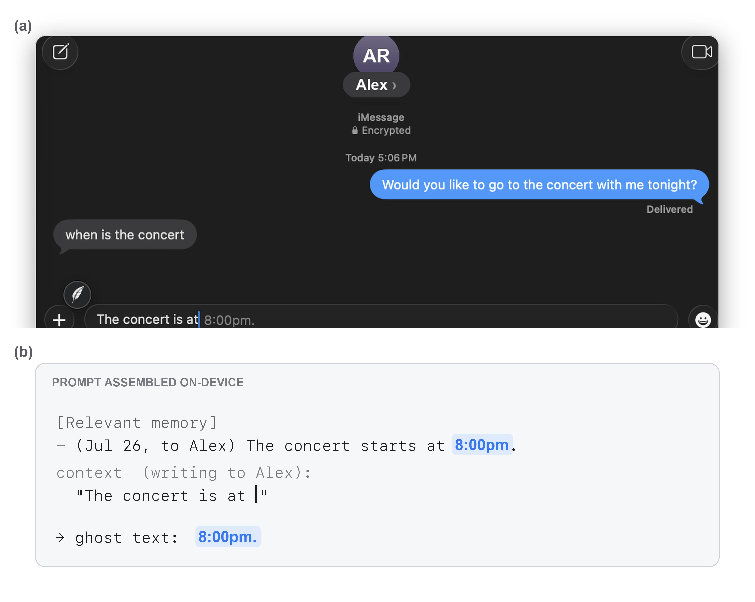
\includegraphics[width=\columnwidth]{figures/teaser.pdf}
\caption{PFM in the deployed autocomplete assistant, with the recipient pseudonymized. The user replies to a question about a concert and types ``The concert is at.'' PFM supplies the remembered time in a compact \texttt{[Relevant memory]} block that is available to the frozen language model when it generates the completion.}
\label{fig:teaser}
\end{figure}

Recent agent-memory systems organize prior interactions through extracted records, temporal graphs, external memory tiers, and associative retrieval \citep{chhikara2025mem0,rasmussen2025zep,gutierrez2024hipporag,packer2023memgpt}. Long-horizon benchmarks such as LongMemEval evaluate whether an assistant can recover information from earlier conversations \citep{wu2024longmemeval}. Real-time personal assistance adds constraints that retrieval accuracy alone does not capture. Similar text may refer to different people, a previously correct fact may become obsolete after an update, and a useful retrieval may arrive after the host model has already started generation. These failures are especially relevant on personal devices, where memory retrieval competes with the language model for limited compute and must operate within an interactive latency budget.

We study this setting as \emph{deadline-constrained personal fact retrieval}. A request contains the local typing context, interaction participants, a personal fact store, a prompt budget, and a serving deadline. The memory layer selects a small set of facts for injection into the prompt. We distinguish misattribution, in which a retrieved fact belongs to the wrong person or entity; staleness, in which an obsolete value is surfaced as current; and lateness, in which otherwise useful context is unavailable by the serving deadline. These errors require evaluation beyond semantic relevance alone.

We propose \textbf{Personal Fact Memory (PFM)} for this setting. PFM stores prompt-ready atomic facts with explicit entity and participant fields and temporal version information. Field-weighted lexical retrieval uses the identities present in the current interaction, and a local entity graph provides an additional association signal when the typed context omits the target entity. Fact extraction and index maintenance run asynchronously, while serving uses only in-memory retrieval and immutable snapshots. No embedding model or language model is invoked on the serving path. When two observations are assigned the same mutable slot key, temporal versioning removes the superseded value from the active index while retaining its history.

We evaluate the memory layer first in isolation and then through the model that consumes its output. In offline replay through the deployed autocomplete data path, PFM places the ground-truth fact in the prompt in 24 of 25 scenarios, and participant-aware retrieval resolves 8 of 8 targeted identity probes against 5 of 8 without the participant field. On a controlled 240-query update benchmark spanning revision depth, paraphrase, cancellation, and identity ambiguity, keyed supersession recalls the current value on every query with zero stale exposure, where the keyless configuration exposes a superseded value on 66.2\% of queries. Under identical corpus, device, and budget conditions, validity-aware lexical serving is the only family that delivers clean facts within millisecond deadlines: a local MiniLM retriever attains the highest current-value recall of any baseline yet exposes stale values on 77.9\% of requests and misses every deadline below its 15~ms query encoding. Replaying the same prompts through a frozen 7B model shows the differences propagate to text: correct completions rise from 0\% without memory to 92.5\% with PFM, with no stale or wrong-person generations, while plain BM25 yields 35.8\% stale completions. These measurements still do not establish that users accept the resulting completions in live use.

We make three contributions.
\begin{enumerate}
\item \textbf{Problem formulation.} We formulate deadline-constrained personal fact retrieval and define misattribution, staleness, and lateness as distinct retrieval failures under prompt and serving-time budgets.
\item \textbf{Memory architecture.} We develop PFM, which combines participant-aware fact representation, temporal versioning for keyed updates, asynchronous memory construction, and a model-free serving path based on in-memory retrieval and immutable snapshots. We state the conditions under which keyed updates maintain a unique active value and the serving protocol bounds memory-induced delay.
\item \textbf{System evidence.} We evaluate PFM through offline replay and mechanism probes in a deployed autocomplete assistant; a controlled update benchmark that measures current-fact recall, stale exposure, and co-injection under keyed revision, paraphrase, and cancellation; baseline comparisons against BM25 variants, a local dense retriever, and a hybrid under identical corpus, device, and deadline budgets, summarized as clean-retrieval rate versus serving deadline; completion-level replay through a frozen local model that measures correct, stale, and wrong-person generations and time to first token; and scaling measurements from 100 to 100{,}000 facts with fixed hardware and stated timing boundaries.
\end{enumerate}

\section{Related Work}

\paragraph{Personal and evolving memory.} Long-term agent memory has been implemented through external stores, structured records, and graph-based retrieval. MemGPT manages bounded context by moving information between memory tiers \citep{packer2023memgpt}; Mem0 extracts and updates persistent facts \citep{chhikara2025mem0}; A-MEM stores linked atomic notes \citep{xu2025amem}; and HippoRAG retrieves through an entity graph \citep{gutierrez2024hipporag}. EMG-RAG is especially relevant to personal assistants because it builds an editable memory graph from smartphone data and applies the resulting memory in a smartphone assistant \citep{wang2024emgrag}. Temporal consistency has also become a direct object of study. Zep maintains a temporal knowledge graph with explicit history \citep{rasmussen2025zep}; APEX-MEM preserves temporal evolution in an append-only property graph and resolves conflicting information during retrieval \citep{banerjee2026apexmem}; Temporal Semantic Memory models event time and durative personal states \citep{su2026tsm}; and Memora evaluates whether personalized agents continue to rely on obsolete information after updates \citep{uddin2026memora}. PFM therefore does not rely on personalization, graph structure, or temporal memory as standalone novelty. Its focus is the retrieval regime of an interactive personal assistant, where identity attribution, current validity, and availability before generation must be satisfied on the same request.

\paragraph{Efficient memory serving.} Recent systems treat the cost of memory operations as part of the design problem. Lightweight LLM Agent Memory separates online retrieval from offline consolidation and operates under a fixed retrieval budget \citep{zhang2026lightmem}. AME targets smartphones directly and co-designs vector-memory querying, insertion, and index maintenance for mobile hardware \citep{zhao2025ame}. AgentIR treats long-term conversational memory as a latency-sensitive retrieval workload and adaptively decides when a dense retrieval channel is worth its cost \citep{yuan2026agentir}. System-level profiling further shows that memory construction, retrieval, and freshness can shift cost across different phases of agent execution \citep{omri2026agentmemory,zhou2026ready}. These systems make latency and resource use explicit, which narrows the claim for PFM. PFM studies a serving path that uses participant metadata and active temporal state, invokes no embedding model or language model at completion time, and falls back to a published snapshot when a fresh retrieval exceeds its waiting budget.

\paragraph{Evaluation of long-term memory.} LoCoMo and LongMemEval evaluate whether an assistant can recover and reason over information from extended interaction histories \citep{maharana2024evaluating,wu2024longmemeval}. More recent work adds temporal validity, obsolete-memory penalties, retrieval efficiency, and phase-level systems cost to this evaluation space \citep{uddin2026memora,su2026tsm,huang2026licomemory,omri2026agentmemory}. The setting studied here adds application context that is specific to continuous autocomplete: the current participant can disambiguate otherwise similar facts, prompt space is limited, and memory must be available before the completion request proceeds. We evaluate these requirements separately through identity errors, stale co-injection, fact availability, and retrieval latency instead of treating long-term memory quality as a single accuracy measure.

\section{Problem Formulation}

We consider a single user whose personal memory evolves as documents, messages, and other observations arrive over time. At time $t$, let $\mathcal{M}_t$ denote the facts retained by the memory layer, including active facts and facts preserved only as history. A completion request consists of typing context $c_t$, a participant set $P_t$, a serving deadline $\Delta_t$, a maximum number of injected facts $k$, and a character budget $B$. The deadline is the latest time at which retrieved context can be incorporated before the host model begins generation.

\begin{definition}[Personal fact]
A stored fact is a tuple
\begin{equation}
f=(z_f,E_f,P_f,\kappa_f,a_f,b_f,\ell_f),
\end{equation}
where $z_f$ is the prompt-ready text, $E_f$ is a set of normalized entities, $P_f$ is the participant set associated with the source, $\kappa_f$ is an optional key for a mutable semantic slot, $[a_f,b_f)$ is the interval during which the system treats the fact as active, and $\ell_f$ is its prompt length. We set $b_f=\infty$ when a fact has not been superseded. The active view at time $t$ is $\mathcal{A}_t=\{f\in\mathcal{M}_t:a_f\le t<b_f\}$.
\end{definition}

The active interval records the state of the memory system; it does not assert that the stored proposition is true in the world. An extractor may fail to recognize that a new observation revises an earlier one. Semantic validity must therefore be evaluated separately from the system's active view.

A retrieval policy $\pi$ maps $(\mathcal{A}_t,c_t,P_t)$ to an ordered set $S_{\pi,t}\subseteq\mathcal{A}_t$ and incurs serving latency $L_{\pi,t}$. The returned set must satisfy
\begin{equation}
|S_{\pi,t}|\le k, \qquad \sum_{f\in S_{\pi,t}}\ell_f\le B,
\end{equation}
and must be available by $\Delta_t$ to affect the current completion. The prompt constraints limit the amount of memory supplied to the language model, while the deadline limits the time available to obtain it.

For evaluation, let $R_t(f)=1$ when fact $f$ is relevant to request $t$, $I_t(f)=1$ when its entity and participant attribution matches the intended identity of the request, and $V_t(f)=1$ when the proposition remains semantically valid at time $t$. These labels describe ground truth and need not be observable by the retrieval policy. Define
\begin{equation}
\mathcal{G}_t=\{f\in\mathcal{M}_t:R_t(f)=1,\ I_t(f)=1,\ V_t(f)=1\}
\end{equation}
as the set of facts that are relevant, correctly attributed, and valid for request $t$.

\begin{definition}[Deadline-constrained personal fact retrieval]
Retrieval succeeds on request $t$ when at least one fact in $\mathcal{G}_t$ is returned within the serving deadline while satisfying the prompt constraints. Define correct-by-deadline availability as
\begin{equation}
Y^{\mathrm{db}}_{\pi,t}=\mathbf{1}\{S_{\pi,t}\cap\mathcal{G}_t\neq\varnothing\}\mathbf{1}\{L_{\pi,t}\le\Delta_t\}.
\end{equation}
\end{definition}

Misattribution occurs when a retrieved fact is relevant in content but belongs to the wrong identity, $E^{\mathrm{id}}_{\pi,t}=\mathbf{1}\{\exists f\in S_{\pi,t}:R_t(f)=1,\ I_t(f)=0\}$. Staleness occurs when a retrieved fact concerns the intended identity but is no longer valid, $E^{\mathrm{stale}}_{\pi,t}=\mathbf{1}\{\exists f\in S_{\pi,t}:R_t(f)=1,\ I_t(f)=1,\ V_t(f)=0\}$. Lateness occurs when retrieval misses the serving deadline, $E^{\mathrm{late}}_{\pi,t}=\mathbf{1}\{L_{\pi,t}>\Delta_t\}$. The three indicators need not be mutually exclusive. A prompt may contain both a current value and a superseded value, so successful fact retrieval does not by itself imply temporal correctness.

For evaluations with complete identity and validity labels, we also define clean correct-by-deadline retrieval,
\begin{equation}
Y^{\mathrm{clean}}_{\pi,t}=Y^{\mathrm{db}}_{\pi,t}\mathbf{1}\{E^{\mathrm{id}}_{\pi,t}=0\}\mathbf{1}\{E^{\mathrm{stale}}_{\pi,t}=0\}.
\label{eq:clean_deadline}
\end{equation}
This stricter outcome requires the target fact to be available by the deadline without exposing a relevant wrong-identity or stale fact on the same request.

\paragraph{Keyed temporal updates.} Consider a mutable semantic slot with key $\kappa$. Suppose every recognized revision to that slot receives the same key and updates are processed serially. When a new fact $f'$ with key $\kappa$ is inserted at time $s$, the update rule sets $a_{f'}=s$ and $b_{f'}=\infty$. If an active predecessor $f$ with the same key exists, the rule also sets $b_f=s$. The predecessor remains in $\mathcal{M}_t$ as history but is removed from the active view.

\begin{proposition}[Unique active value under keyed supersession]
\label{prop:unique_active_value}
Fix a key $\kappa$. If updates with key $\kappa$ are processed serially by the rule above and the store initially contains at most one active fact with that key, then for every time $t$,
\begin{equation}
\left|\{f\in\mathcal{A}_t:\kappa_f=\kappa\}\right|\le 1.
\end{equation}
\end{proposition}

The claim follows by induction over keyed updates because a new value becomes active at the same instant that the unique active predecessor, if any, is closed. The full proof is given in the technical appendix. The result depends on correct key assignment; it does not guarantee that the extractor identifies every revision or that the newest observation is semantically correct.

\section{Personal Fact Memory}

PFM separates memory construction from memory serving. Construction begins after the system observes a document and may include fact extraction, deduplication, temporal updates, graph maintenance, and pruning. These operations run asynchronously. Serving operates on the resulting in-memory state and does not call an embedding model or language model.

\subsection{Memory Construction}

Each extracted fact carries prompt text, normalized entities, source participants, and an optional key for a mutable semantic slot, as defined in the previous section. In the deployed assistant, the participant field is obtained from the interaction context in which the source document is observed. For supported messaging and mail applications, the active window identifies the interlocutor independently of the words in the document. This metadata is stored with the fact and later used during retrieval.

When a newly extracted fact receives the same slot key as an active fact, PFM applies keyed supersession and removes the predecessor from the active view. Supersession is checked before near-duplicate admission control: a revision that reuses the sentence surface with only the value changed must update the slot, not be absorbed as a re-observation of the old fact. Only an exactly repeated sentence reinforces the current value. Facts for which no reliable slot key is available remain separate observations. Proposition~\ref{prop:unique_active_value} therefore applies to recognized revisions, not to arbitrary pairs of contradictory text.

PFM maintains a fielded inverted index over active facts, with separate fields for prompt text, entities, and participants. It also maintains an entity co-occurrence graph whose edges summarize associations observed in the user's fact store. Index and graph updates occur on the construction path. Historical facts may be retained for provenance, but inactive facts do not enter retrieval.

The implementation also records a fact class and a usage score. Facts are labeled episodic, semantic, or profile for retention purposes. Profile facts are pinned, while other facts may be pruned as recency and use decline. The usage score increases when a completion that used the fact is accepted and decays over time. These quantities are used as ranking and retention signals; the paper does not treat them as evidence for a cognitive model of human memory.

\subsection{Retrieval and Ranking}

For a completion request, PFM constructs a focal query from the tokens preceding the cursor and from the current participant set. Token weights decay with distance from the cursor as $\lambda^d$, with $\lambda=0.95$ in the deployed configuration. Participant terms receive an additional weight of $1.5$, and the query retains at most 12 terms ranked by weighted inverse document frequency. Limiting the query size bounds the amount of query-side work before index traversal.

The lexical retriever uses BM25F \citep{robertson2004simple,robertson2009probabilistic} over the text, entity, and participant fields. The deployed field weights are $1.0$, $2.5$, and $2.0$, respectively. Participant weighting distinguishes facts whose text is similar but whose source interactions involve different people. For example, two messages that both say ``deadline moved to Friday'' can be separated when one was sent to Alice and the other to Bob.

Lexical retrieval is supplemented by bounded one-hop propagation over the entity graph. Let $Q_t$ be the seed entities recovered from the query and participant metadata, and let $w_{eg}(t)$ be the current weight between entities $e$ and $g$. For fact $f$ with entity set $E_f$, PFM computes
\begin{equation}
s_{\mathrm{assoc}}(f\mid Q_t)=\sum_{e\in Q_t}\sum_{g\in E_f}w_{eg}(t),
\end{equation}
with fixed limits on the number of seeds and neighbors traversed. The graph score provides an association signal when the current text names an entity connected to the target fact but does not name the target directly. This differs from full graph ranking methods such as HippoRAG \citep{gutierrez2024hipporag}, which perform broader propagation for open-domain retrieval.

The deployed ranker combines lexical relevance, recency, prior use, and graph association. Let $\Delta t_f$ denote the age of fact $f$, let $h_f(t)$ denote its decaying usage score, and let $T_{\mathrm{rec}}$ be the recency half-life. The score is
\begin{equation}
\mathrm{score}(f)=\mathrm{BM25F}(q_t,f)\left(\varepsilon+(1-\varepsilon)2^{-\Delta t_f/T_{\mathrm{rec}}}\right)\left(1+\eta h_f(t)\right)+\gamma s_{\mathrm{assoc}}(f\mid Q_t),
\label{eq:pfm_score}
\end{equation}
where $\varepsilon$, $\eta$, and $\gamma$ are fixed parameters. The recency floor $\varepsilon$ allows an old fact to remain retrievable when its lexical evidence is strong. The usage term gives more weight to facts that have previously contributed to accepted completions. The experiments ablate these components separately rather than assuming that each improves retrieval.

PFM ranks candidate facts by \eqref{eq:pfm_score} and inserts them in score order until either $k$ facts or $B$ characters have been selected. This greedy rule is the policy used by the deployed system. The selection problem is not modeled as a user choice problem because users observe and accept a generated completion, not the individual facts that produced it.

\subsection{Serving Protocol}

PFM supports snapshot serving and fresh retrieval with bounded waiting. In snapshot mode, a background thread retrieves candidate facts during typing pauses and publishes an immutable result by atomic pointer replacement. When a completion request arrives, the serving thread reads the latest published snapshot and proceeds without waiting for a new retrieval. In fresh mode, the request starts a new retrieval and waits for at most $\delta_t$ before falling back to the latest snapshot. The waiting budget $\delta_t$ is chosen below the request deadline $\Delta_t$.

Let $r$ be an upper bound on the time required to read a published snapshot after the serving thread is scheduled. Assume that published snapshots are immutable, publication uses an atomic pointer replacement, and the serving path acquires no lock held by memory construction or background retrieval.

\begin{proposition}[Bound on memory-induced waiting]
\label{prop:waiting_bound}
Under the assumptions above, snapshot mode adds at most $r$ time to the completion path. Fresh mode adds at most $\delta_t+r$. These bounds do not depend on the duration of fact extraction, index maintenance, graph updates, or pruning.
\end{proposition}

The bound follows because snapshot mode performs only the bounded snapshot read, while fresh mode waits for at most $\delta_t$ before using a fresh result or the latest snapshot. The full proof is given in the technical appendix. Proposition~\ref{prop:waiting_bound} bounds delay introduced by memory serving; it does not guarantee that a fresh result is available by the deadline or that the retrieved facts are correct.

\paragraph{Pruning.} Periodic pruning removes nonprofile facts whose recency and usage scores fall below a configured threshold and deletes the corresponding graph state. This policy reduces inactive or rarely used state in practice, but a threshold rule alone does not impose a deterministic upper bound on memory size under arbitrary arrival patterns. Storage footprint is therefore measured empirically rather than claimed as a consequence of the pruning rule.

\section{Budgeted Memory Selection}

PFM retrieval produces a candidate set before prompt assembly. The deployed policy orders candidates by the retrieval score in Eq.~\eqref{eq:pfm_score} and inserts facts until the fact-count or character budget binds. This rule is inexpensive, but it can waste prompt capacity when high-scoring facts differ substantially in length. We therefore consider a separate selection problem over the candidate set, without interpreting the candidates as objects of user choice.

Let $C_t$ denote the candidate set for request $t$. Each candidate fact $f\in C_t$ has prompt length $\ell_f$ and a nonnegative value $v_t(f)$ supplied by the retrieval layer. The value may be the deployed PFM score or another predictive score computed from the same candidate features. Conditional on these values, the selector solves
\begin{equation}
S_t^*\in\arg\max_{S\subseteq C_t}\sum_{f\in S}v_t(f)\qquad\text{s.t.}\qquad |S|\le k,\quad \sum_{f\in S}\ell_f\le B.
\label{eq:budgeted_selection}
\end{equation}
The optimization separates retrieval from prompt allocation. Retrieval determines which facts are plausible and how valuable they are; selection determines which of those facts consume the limited prompt budget. The formulation does not require a probabilistic interpretation of $v_t(f)$ and does not assume that the user chooses among retrieved facts.

When lengths are measured in integer characters, Eq.~\eqref{eq:budgeted_selection} is a cardinality-constrained knapsack problem. Index the $n=|C_t|$ candidates by $1,\ldots,n$, and let $D(j,b,m)$ denote the largest total value attainable using the first $j$ candidates, at most $b$ characters, and at most $m$ facts. The recursion is
\begin{equation}
D(j,b,m)=\max\left\{D(j-1,b,m),\;D(j-1,b-\ell_j,m-1)+v_t(j)\right\},
\label{eq:selection_dp}
\end{equation}
where the second term is omitted when $b<\ell_j$ or $m=0$.

\begin{proposition}[Exact budgeted selection]
\label{prop:budgeted_selection}
For nonnegative candidate values and integer fact lengths, the dynamic program in Eq.~\eqref{eq:selection_dp} returns an optimal solution to Eq.~\eqref{eq:budgeted_selection} in $O(|C_t|Bk)$ time and $O(Bk)$ memory. If all candidate lengths are equal and the character budget permits at least $k$ facts, the solution reduces to selecting the $k$ candidates with largest values.
\end{proposition}

The recursion conditions on whether the final candidate is excluded or included, which yields optimal substructure; rolling the candidate dimension gives the stated memory bound. A full proof is given in the technical appendix. In the deployed configuration, $k=6$ and $B=800$ characters, and the retrieval stage produces a shortlist of roughly 40 candidates. The deployed assistant continues to use greedy score order; the exact selector of Proposition~\ref{prop:budgeted_selection} is evaluated separately as a secondary policy. Because completion acceptance is observed only after the language model transforms the prompt into a completion, this paper does not interpret candidate values as structural preference parameters.

\section{Deployment Setting}

PFM is integrated into a commercially deployed macOS autocomplete assistant. The assistant provides inline completions in text fields across applications: a continuation appears at the cursor as ghost text, the user can accept the full completion or a single word, and continued typing dismisses the suggestion. This interaction makes the serving constraint concrete because memory must be incorporated before the prompt is handed to the host model for the current completion. Acceptance also provides an observable usage signal for the memory supplied on that request.

\paragraph{Participant context.} For supported messaging and mail applications, the frontmost window exposes the interlocutor through its title. PFM records this value as participant metadata when a sent message is observed and uses the current window title again when a later completion request is issued. The participant signal is therefore obtained from the interaction context rather than inferred only from the words being typed. This metadata instantiates the participant set $P_t$ in the retrieval problem and allows two lexically similar facts to be distinguished when they arose in conversations with different people.

\paragraph{Memory acquisition.} The assistant observes sent text after a send-confirmation event and on relevant application or window transitions. Observations are passed asynchronously to memory construction, so extraction, indexing, temporal updates, graph maintenance, and pruning do not delay the completion request that triggered capture. The deployment excludes password and secure-entry fields, suppresses capture from credential-management applications, and drops content that matches secret-like patterns such as API keys or access tokens. The retained fact store remains on the device.

\paragraph{Prompt integration.} At completion time, PFM serializes the selected facts into a compact \texttt{[Relevant memory]} block in the user-context portion of the prompt. The block is capped at the character budget $B$, so memory cannot displace more than the allotted amount of live context. In snapshot mode, the same published memory block can be reused during a typing burst. A stable block avoids changing the prompt prefix at every keystroke and can preserve prompt caching when the host model supports it. In fresh mode, retrieval waits only for the budget specified in the serving protocol and otherwise falls back to the latest snapshot.

\paragraph{Usage feedback.} Acceptance is recorded after the user adopts a completion, rather than when a fact is merely retrieved. An accepted completion triggers the usage update associated with memory supplied for that request, while a dismissed completion does not reinforce those facts. The resulting signal is used by the retention and ranking mechanisms described above. We treat acceptance as a usage signal, not as direct evidence that any particular retrieved fact caused the completion to be accepted.

\section{Evaluation}

We evaluate PFM at the memory layer using replay through the deployed assistant's capture and serving paths, and then extend the evaluation along four axes that replay alone cannot support: temporal correctness on a controlled update benchmark, comparison against standard retrieval families under identical corpus, device, and deadline budgets, completion-level effects through a frozen local language model, and systems scaling on a fixed hardware profile. The primary replay metric is target fact availability, defined as the fraction of requests for which the prompt contains the ground-truth tokens. This metric is weaker than the clean correct-by-deadline outcome in Eq.~\eqref{eq:clean_deadline} because the replay corpus does not provide exhaustive identity and validity labels for every retrieved candidate. We therefore report targeted identity and stale co-injection probes separately rather than constructing an unsupported clean aggregate.

\subsection{Replay Setup}

A scripted 28-day sequence of sent messages is ingested through the deployed capture path, including the same participant metadata used by the application (Table~\ref{tab:harness}). The small harness contains 8 indexed facts and 7 completion scenarios. The large harness begins with 31 hand-written seed facts, adds 16 chit-chat messages and 240 synthetic filler messages, and produces 270 indexed facts. The 25 large-harness scenarios contain 20 direct recalls of a date, amount, or identifier; two associative recalls in which the typed prefix omits the target entity; one conflicting-update case; one CJK entity case; and one extraction case designed to omit the signal verb required by the rule extractor. Retrieval uses $k=6$ and an 800-character prompt budget.

\begin{table}[t]
\centering
\small
\begin{tabular}{@{}lrrr@{}}
\toprule
Harness & Messages & Facts indexed & Scenarios \\
\midrule
Small & 9 & 8 & 7 \\
Large & 287 & 270 & 25 \\
\bottomrule
\end{tabular}
\caption{Replay harnesses used in the current evaluation. The large harness contains 31 seed messages, 16 chit-chat messages, and 240 synthetic fillers.}
\label{tab:harness}
\end{table}

\subsection{Target Fact Availability}

Table~\ref{tab:availability} compares the same replay requests with and without memory. With PFM enabled, the target tokens reach the prompt in 6 of 7 small-harness scenarios and 24 of 25 large-harness scenarios. With memory disabled, none of the target facts are present in the prompt because the live typing context does not contain them. On the large harness, availability is 20/20 for direct recall, 2/2 for the associative cases, 1/1 for the conflicting-update case, and 1/1 for the CJK case. The designed extraction failure accounts for the remaining miss.

\begin{table}[t]
\centering
\small
\begin{tabular}{@{}lcc@{}}
\toprule
Harness & Memory on & Memory off \\
\midrule
Small & 6/7 (86\%) & 0/7 (0\%) \\
Large & 24/25 (96\%) & 0/25 (0\%) \\
\bottomrule
\end{tabular}
\caption{Target fact availability in replay. Availability records whether the ground-truth tokens appear in the constructed prompt; it does not by itself rule out stale or misattributed co-injection.}
\label{tab:availability}
\end{table}

The write path admits 30 of 31 seed facts and none of the 16 chit-chat messages in this scripted corpus. The missed seed is a sentence without the signal verb required by the deployed rule extractor. These counts characterize extraction on the replay corpus only and should not be interpreted as general extraction precision or recall.

\subsection{Identity Attribution}

The overall availability metric does not test whether lexically similar memories are assigned to the correct person. We therefore construct four pairs of near-identical facts associated with different participants and query each pair from both participant contexts, yielding eight identity probes. PFM resolves all 8 probes when participant metadata is retained. Removing the participant field and its retrieval weight reduces performance to 5/8. Overall availability on the original 25 scenarios remains 24/25 in both conditions, showing why identity-specific probes are needed in addition to aggregate availability.

\subsection{Retrieval Latency}

Latency is measured in a release build on Apple Silicon with a single retrieval thread. At 270 facts, median retrieval time is 0.011~ms, p95 is 0.024~ms, and the maximum across 500 runs is 0.109~ms. In a 20{,}000-fact stress store, median retrieval time is 1.81~ms and p95 is 2.03~ms. Table~\ref{tab:latency} reports these measurements. The 20{,}000-fact result establishes performance for the tested store and implementation; it is not a claim about asymptotic scaling.

\begin{table}[t]
\centering
\small
\begin{tabular}{@{}lrrr@{}}
\toprule
Scale & p50 & p95 & max \\
\midrule
270 facts, 500 runs & 0.011~ms & 0.024~ms & 0.109~ms \\
20{,}000 facts & 1.81~ms & 2.03~ms & n/a \\
\bottomrule
\end{tabular}
\caption{Retrieval latency in the deployed implementation. Measurements are from a release build on Apple Silicon using a single retrieval thread.}
\label{tab:latency}
\end{table}


\subsection{Temporal Correctness under Keyed Revision}

The replay harness contains a single conflicting-update scenario, which is too small to estimate temporal error rates. We therefore construct a controlled update benchmark of 160 revision chains over (entity, slot) pairs drawn from 36 people and 20 projects, with six mutable slot types (meeting time, deadline, launch date, day rate, budget cap, room). Each chain applies zero to four revisions with distinct values; messages rotate through three sentence templates and queries through two phrasings; roughly ten percent of revised chains repeat the identical sentence surface with only the value changed; and 25 percent of eligible chains end in cancellation rather than replacement. Six shared-first-name pairs are assigned chains on the same slot so that the query surface form is ambiguous while the underlying keys differ. Every value token is globally unique, so exposure metrics reduce to exact normalized containment. This yields 240 labeled queries per corpus, evaluated at two corpus sizes (with and without 1{,}000 filler messages) and two prompt budgets; we report 95 percent Wilson intervals.

Two arms isolate the supersession mechanism. The \emph{keyed} arm uses a key-emitting rule extractor (entity and slot noun plus a type-consistent value) with supersession applied before near-duplicate admission, as described in the construction section. The \emph{keyless} arm ingests the same sentences with keys stripped, which is the configuration whose limitation the conflicting-update scenario exposed. Extraction coverage is identical by construction, so differences are attributable to temporal versioning alone.

\begin{table}[t]
\centering
\small
\begin{tabular}{@{}llrrrr@{}}
\toprule
Arm & $B$ & Current & Stale & Co-inj. & Clean \\
\midrule
Keyed   & 800 & 1.000 & .000 & .000 & .875 \\
Keyless & 800 & .812  & .662 & .525 & .283 \\
Keyed   & 240 & .896  & .000 & .000 & .896 \\
Keyless & 240 & .667  & .388 & .250 & .417 \\
\bottomrule
\end{tabular}
\caption{Update benchmark (240 labeled queries, filler corpus; the no-filler corpus is within one point on every entry). Current = current-value recall; Stale = stale-fact exposure; Co-inj.\ = current and superseded values in the same prompt; Clean = current value present with no stale or wrong-person exposure. The 95 percent upper bound on keyed stale exposure is 1.6 percent.}
\label{tab:temporal}
\end{table}

Table~\ref{tab:temporal} shows that keyed supersession changes temporal behavior end to end. The keyed arm recalls the current value on all 240 queries and never exposes a superseded value, so co-injection is eliminated rather than reduced. The keyless arm exposes a stale value on 66.2 percent of queries and co-injects on 52.5 percent, and recency ordering does not repair this because both values often survive the top-$k$ cut. Three further effects are worth recording. First, near-duplicate admission interacts destructively with verbatim revisions: in the keyless arm only 87.1 percent of current values are indexed at all, and on the verbatim-revision slice current-value recall drops to .214 because the revised sentence is absorbed as a re-observation of the old fact. Checking supersession before deduplication removes this failure. Second, cancellations are the worst case for the keyless arm, which continues to surface the cancelled time on 85.7 percent of those queries; the keyed arm returns the cancellation statement instead. Third, the tight budget suppresses some stale exposure in the keyless arm (.388 versus .662) only by truncating facts of every kind, including current ones (.667 recall); budget pressure is not a staleness defense. The keyed arm's residual errors are wrong-person exposures (.125 at $B{=}800$, .000 at $B{=}240$), concentrated on the engineered ambiguous queries, where the correct fact ranks first but a same-first-name competitor also enters one of the six slots. Identity exposure under ambiguity, not staleness, is the remaining failure mode; the completion-level study below measures its downstream effect.

\subsection{Retrieval Baselines under the Serving Deadline}

We next compare PFM against standard retrieval families on the same corpus, device, and budgets, using the update benchmark's filler corpus (1{,}160 active facts plus retained superseded facts for validity-agnostic arms) with $k{=}6$ and $B{=}800$. The arms are: plain text BM25 over all facts; BM25 with PFM's recency decay; BM25 restricted to currently valid facts (the same update information PFM uses, without field weighting); a dense retriever using all-MiniLM-L6-v2 running locally on the same CPU, with corpus embeddings precomputed at build time and only query encoding on the serving path; a sparse-plus-dense hybrid fused by reciprocal rank fusion; and PFM in fresh and snapshot modes. Latency is the median of three timed runs per query after a warmup pass, measured around the full retrieval call on a single thread.

\begin{table}[t]
\centering
\small
\begin{tabular}{@{}lrrrrr@{}}
\toprule
Method & Clean & Curr. & Stale & p50 & p95 \\
 & & & & (ms) & (ms) \\
\midrule
PFM (fresh)      & \textbf{.875} & 1.000 & .000 & 0.06 & 0.09 \\
PFM (snapshot)   & \textbf{.875} & 1.000 & .000 & $\approx$0 & $\approx$0 \\
BM25 + validity  & .758 & .892 & .000 & 0.02 & 0.03 \\
BM25 + recency   & .212 & .863 & .633 & 0.04 & 0.08 \\
BM25             & .188 & .858 & .692 & 0.03 & 0.06 \\
Dense (MiniLM)   & .196 & .975 & .779 & 15.4 & 37.1 \\
Hybrid (RRF)     & .192 & .879 & .771 & 14.8 & 30.1 \\
\bottomrule
\end{tabular}
\caption{Retrieval baselines on the update benchmark under identical corpus, device, and budgets. Clean intervals: PFM (.827, .911); BM25+validity (.700, .808); all validity-agnostic arms are below .27. Dense corpus encoding at build time takes 13.7~s; the reported latency is query-side only.}
\label{tab:baselines}
\end{table}

\begin{figure}[t]
\centering
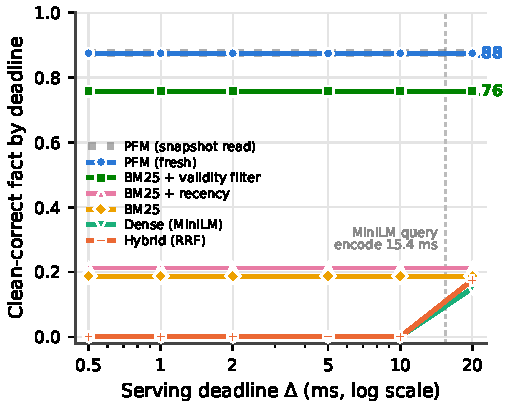
\includegraphics[width=\columnwidth]{figures/deadline_curve.pdf}
\caption{Fraction of requests that obtain a clean correct fact within a serving deadline $\Delta$, on the update benchmark. Validity-aware lexical serving is deadline-insensitive across the interactive range; the snapshot path is deadline-independent by construction and its curve coincides with PFM (fresh) at these deadlines; the local dense retriever cannot meet any deadline below its query-encoding cost (p50 15.4~ms) regardless of ranking quality.}
\label{fig:deadline}
\end{figure}

Table~\ref{tab:baselines} and Figure~\ref{fig:deadline} support three conclusions. First, temporal correctness is determined by the write path, not the ranker: the two validity-aware arms reach clean rates of .875 and .758, while every validity-agnostic arm is below .27 regardless of retrieval family. Giving plain BM25 the same validity bits recovers most of the gap; PFM's field weighting contributes the remainder, raising current-value recall from .892 to 1.000, largely on the associative and participant-dependent queries. Second, representational power does not substitute for temporal state: the dense retriever attains the best current-value recall of any baseline (.975) and the worst stale exposure (.779), because embedding similarity ranks every version of a revised fact near the query. Third, the deadline dimension separates methods that accuracy alone cannot: MiniLM query encoding costs 15.4~ms at the median on this hardware, so the dense and hybrid arms deliver a clean fact within a 10~ms deadline on zero requests, and within 20~ms on fewer than 18 percent, while PFM's fresh path serves its full clean rate from 0.5~ms and the snapshot path is deadline-independent by construction. On this benchmark, deadline-constrained clean retrieval is achieved only by combining validity-aware construction with a serving path whose cost is below the deadline.

\subsection{Completion-Level Evidence with a Frozen Local Model}

Fact availability establishes that information reached the prompt, not that it changed the completion. We therefore replay a stratified sample of 120 benchmark queries (weighted toward revised and ambiguous chains) through a frozen local model, qwen2:7b served by ollama on the same machine, with temperature 0 and identical decoding across arms. Each request assembles the same prompt the assistant would use---typing context, participant, and the arm's retrieved memory block---and the generated completion is judged by normalized containment: \emph{correct} when it contains the current value, \emph{stale} when it instead contains a superseded value, \emph{wrong-person} when it contains a same-first-name competitor's value, and \emph{other} otherwise. We also record time to first streamed token (TTFT).

\begin{table}[t]
\centering
\small
\begin{tabular}{@{}lrrrrr@{}}
\toprule
Memory & Correct & Stale & Wrong & Other & TTFT \\
 & & & pers. & & p50 (ms) \\
\midrule
None        & .000 & .000 & .000 & 1.000 & 296 \\
PFM         & \textbf{.925} & .000 & .000 & .075 & 1194 \\
BM25 (plain) & .517 & .358 & .008 & .117 & 1036 \\
\bottomrule
\end{tabular}
\caption{Frozen-LLM replay (qwen2:7b, 120 queries, temperature 0). Correct CI for PFM: (.864, .960); stale CI for plain BM25: (.278, .447). The upper bound on PFM stale and wrong-person generations is 3.1 percent.}
\label{tab:llm}
\end{table}

Table~\ref{tab:llm} shows that prompt-side differences propagate to generations. Without memory, the model produces the labeled value on none of 120 requests; every completion is a guess. With PFM's block, 92.5 percent of completions contain the current value and none contain a stale or wrong-person value. With plain BM25's block, 51.7 percent are correct and 35.8 percent reproduce a superseded value: stale facts in the prompt become stale text in the output at a rate close to the block's stale-exposure rate. Two further observations matter. First, wrong-person exposure does not translate into wrong-person generation for PFM: although a same-first-name competitor's fact enters the prompt on 12.5 percent of benchmark queries, the model selects the correctly attributed fact in every sampled case, plausibly because block lines carry explicit ``to \emph{person}'' attribution and the correct fact ranks first. Prompt-level exposure and completion-level error are related but not identical, which is why both are reported. Second, the memory block has a measurable serving cost at the model: TTFT rises from 296~ms without memory to about 1.2~s with an 800-character block on this 7B CPU configuration, quantifying the prefill price of injected context and motivating the budgeted selection studied next. These results are specific to one model, one decoding configuration, and a containment judge; they establish that retrieved facts change completions, not that users accept them.

\subsection{Budgeted Selection under Synthetic Response Models}

We evaluate budgeted selection in a synthetic response experiment that isolates the allocation rule. The top-$k$ arm and the exact budgeted arm use the same per-user candidate values, $v_t(f)=\exp(\theta_u^{\top}x_t(f))$, where $x_t(f)$ contains lexical relevance, age, usage, graph association, and an intercept. The parameters are updated online from simulated accept or reject feedback. Each configuration runs 1{,}200 episodes with a 25 percent warm-up period over three personas and two seeds. Simulated responses follow MNL, mixed-logit, or nested-logit models. The experiment tests prompt allocation under controlled response functions; it does not identify a model of real user acceptance.

\begin{table}[t]
\centering
\small
\begin{tabular}{@{}lrrrr@{}}
\toprule
& \multicolumn{2}{c}{Top-$k$} & \multicolumn{2}{c}{Budgeted} \\
Response model & Accept. & Chars. & Accept. & Chars. \\
\midrule
MNL & .788 & 198 & .776 & 166 \\
Mixed logit & .732 & 200 & .717 & 168 \\
Nested logit & .785 & 199 & .774 & 166 \\
\bottomrule
\end{tabular}
\caption{Synthetic comparison under the binding $B=240$ character budget. Both policies use the same learned candidate values. Acceptance is the true probability under the simulated response model, averaged over three personas and two seeds.}
\label{tab:budgeted_selection_sim}
\end{table}

Under the binding budget (Table~\ref{tab:budgeted_selection_sim}), exact selection uses 31 to 33 fewer characters than top-$k$, a reduction of approximately 16 to 17 percent, while simulated acceptance is lower by 1.1 to 1.5 percentage points. When $B=800$, the character budget does not bind and the exact selector coincides with top-$k$ under the same learned values. The simulation shows a prompt-allocation tradeoff under synthetic response models: budget-aware selection reduces prompt use when capacity is tight, with a small reduction in modeled response probability. It does not establish that the same tradeoff holds for generated completions or real user acceptance.

\subsection{Scaling Measurements}

Table~\ref{tab:scaling} reports systems measurements for the reference implementation across store sizes from 100 to 100{,}000 facts. Each row builds a fresh store from synthetic facts whose entity pool grows with store size, so shared vocabulary terms produce posting lists that grow with the store; this distribution is deliberately denser than the replay corpus. Hardware and measurement boundaries are fixed: Apple M2, 8 cores, 16~GB RAM, macOS~26.5, CPython~3.11, single retrieval thread, warm process, timing by a monotonic counter around the full retrieval call (query construction, scoring, ranking, and block formatting), with the first 50 queries discarded as warmup. Per-fact update cost is measured around each insertion, including deduplication, supersession, index, and graph updates.

\begin{table}[t]
\centering
\small
\begin{tabular}{@{}rrrrrr@{}}
\toprule
Facts & p50 & p95 & p99 & Add p50 & RSS \\
 & (ms) & (ms) & (ms) & (ms) & (MB) \\
\midrule
100     & 0.18 & 0.20 & 0.21 & 0.019 & 1.3 \\
1{,}000  & 0.71 & 0.83 & 0.99 & 0.061 & 1.8 \\
5{,}000  & 3.02 & 7.75 & 21.5 & 0.100 & 13.1 \\
10{,}000 & 5.47 & 6.01 & 6.31 & 0.096 & 13.2 \\
20{,}000 & 12.5 & 16.8 & 22.5 & 0.098 & 32.0 \\
50{,}000 & 36.8 & 43.3 & 45.2 & 0.099 & 105.9 \\
100{,}000 & 81.1 & 94.1 & 113.5 & 0.101 & 98.2 \\
\bottomrule
\end{tabular}
\caption{Reference-implementation scaling on a dense synthetic term distribution (Apple M2, single thread). RSS is the process-memory delta around the build and is approximate at large sizes due to allocator reuse. Ingest throughput is 8{,}800--43{,}600 facts/s across the grid; a full prune pass takes 1.55~s at 100{,}000 facts.}
\label{tab:scaling}
\end{table}

Three observations follow. First, per-fact update cost is essentially flat (about 0.1~ms from 5{,}000 facts onward), so construction-path throughput does not degrade with store size in this range. Second, fresh-retrieval latency grows roughly linearly with posting-list length: the same implementation that serves 1.81~ms at 20{,}000 facts on the replay distribution (Table~\ref{tab:latency}) reaches 12.5~ms at 20{,}000 facts and 81~ms at 100{,}000 facts on the dense synthetic distribution. Latency at scale is therefore a property of term-frequency structure, not of fact count alone. Third, the serving protocol changes what these numbers mean for the product: snapshot serving keeps the completion path at a single bounded read regardless of store size (Proposition~\ref{prop:waiting_bound}), at the cost of snapshot staleness, while fresh retrieval beyond roughly 20{,}000 dense facts requires index-side mitigation such as posting-list truncation or impact ordering. We report both regimes rather than presenting the favorable one.

\subsection{Mechanism Probes and Current Limitations}

Table~\ref{tab:ablation} removes individual retrieval components on the large harness. Removing participant metadata leaves aggregate availability unchanged but reduces the targeted identity score from 8/8 to 5/8. Removing the entity graph or recency decay also leaves aggregate availability at 24/25. The two associative scenarios therefore do not isolate a case in which graph propagation is necessary, and the current replay does not establish an availability benefit from recency decay. Recency-only and random-$k$ retrieval each recover 1 of 25 target facts, which confirms that the full result is not produced by these degenerate policies.

\begin{table}[t]
\centering
\small
\begin{tabular}{@{}lccc@{}}
\toprule
Variant & Availability & Identity & Stale co-injection \\
\midrule
PFM & 24/25 & 8/8 & yes \\
No participants & 24/25 & 5/8 & yes \\
No entity graph & 24/25 & 8/8 & yes \\
No recency decay & 24/25 & 8/8 & yes \\
Recency only & 1/25 & n/a & n/a \\
Random $k$ & 1/25 & n/a & n/a \\
\bottomrule
\end{tabular}
\caption{Mechanism probes on the large replay harness. Identity reports the eight targeted participant-disambiguation probes. Stale co-injection records whether the superseded value also reaches the prompt in the conflicting-update scenario.}
\label{tab:ablation}
\end{table}

The conflicting-update scenario in this replay exposes the keyless configuration: without a slot key, the newer value is retrieved (the scenario counts as available) but the superseded value is also injected. The update benchmark quantifies this failure at scale (52.5 percent co-injection over 240 queries) and shows that the key-emitting extractor with supersession-before-deduplication eliminates it (Table~\ref{tab:temporal}). The scope of the guarantee is unchanged: temporal consistency follows after a revision has been assigned the correct key, not from textual contradiction alone, and the benchmark's slot patterns share a template family with its generator. Key assignment on unconstrained natural text remains open, and the shipped Swift extractor has not yet adopted the key-emitting rules evaluated here.

The present evaluation measures the behavior of the memory layer before generation. It does not establish that the language model uses the retrieved fact correctly or that memory improves user acceptance, and the scripted replay is smaller and cleaner than a long-running personal corpus. These distinctions bound the claims supported by the current experiments.

\section{Limitations}

The controlled evidence in this paper stops short of live product impact. The update benchmark, the baseline comparison, and the frozen-model replay are built from template-generated corpora whose value tokens are globally unique by construction; real personal text is noisier, and paraphrase in the benchmark spans a fixed template family rather than unconstrained rewording. The completion-level study uses one frozen model, one decoding configuration, and a normalized-containment judge; it establishes that retrieved facts change generated text, not that users accept the resulting completions or benefit over long-running personal histories.

Temporal versioning depends on the construction path recognizing that two observations refer to the same mutable slot. The key-emitting extractor evaluated here achieves this on the benchmark's six slot types, and correcting its slot detection required value-type constraints precisely because noun families overlap across slots---evidence that key assignment is the fragile step. Proposition~\ref{prop:unique_active_value} characterizes consistency after revisions receive a common key; it does not guarantee revision detection on unconstrained natural text, and the extractor shipped in the deployed assistant has not yet adopted the keyed rules, so deployed behavior currently matches the keyless arm of Table~\ref{tab:temporal}.

Several components remain only partially identified, and the systems numbers carry stated scope. Removing the entity graph or recency decay does not change availability on the 25 replay scenarios, so their necessity is not established there. Under identity ambiguity with $k{=}6$ slots, a same-first-name competitor's fact still enters the prompt on 12.5\% of benchmark queries even though the frozen model selected the correctly attributed fact in every sampled case; exposure-level ambiguity is unresolved at the retrieval layer. The scaling grid shows that fresh-retrieval latency is governed by term-frequency structure rather than fact count alone, reaching 81~ms at 100{,}000 dense synthetic facts in the reference implementation; snapshot serving hides this from the completion path but not from snapshot freshness, and index-side mitigation at that scale is future work. All latency measurements are from one Apple Silicon machine with a single retrieval thread.

\section{Conclusion}

We formulated deadline-constrained personal fact retrieval, in which a personal memory layer must return relevant information that is correctly attributed, still valid, and available before generation begins. PFM addresses this setting with participant-aware atomic facts, keyed temporal supersession applied before duplicate admission, asynchronous memory construction, and an in-memory serving path that does not invoke an embedding model or language model. The evaluation supports three conclusions. Temporal correctness is a property of the write path: keyed supersession takes stale exposure from 66.2\% to zero on a 240-query update benchmark, and even plain BM25 recovers most of the clean-retrieval gap when given the same validity information, while no validity-agnostic retriever exceeds a .27 clean rate. The serving deadline separates methods that accuracy alone cannot: a local dense retriever with the best current-value recall of any baseline delivers zero clean facts within a 10~ms deadline because of its query-encoding cost, while PFM serves its full clean rate from 0.5~ms and its snapshot path is deadline-independent by construction. Finally, prompt-side correctness propagates to generations: with a frozen 7B model, correct completions rise from 0\% to 92.5\% with PFM and stale prompts become stale text for validity-agnostic retrieval. Personal memory should therefore be evaluated for misattribution, staleness, and lateness separately, at both the prompt and the completion level, rather than through retrieval accuracy alone.

% % ==========================================================================
% % Ethics / reproducibility notes (AAAI allows an unnumbered statement;
% % check the kit for the current required placement).
% % ==========================================================================

% \paragraph{Ethical Statement.}
% PFM stores personal facts extracted from a user's own writing. The
% deployed system keeps all memory on device, never uploads the store,
% excludes password/secure fields, blocklists credential managers, and
% drops secret-shaped content at capture time. Forgetting is not only a
% resource policy but a privacy property: unreferenced facts decay out of
% the store. \todo{Expand per AAAI-27 ethics-statement guidance; mention
% replay corpora contain no real user data.}

% \paragraph{Reproducibility.}
% All Study-1, Study-3, and Study-4 numbers are reproducible from the
% submitted supplement: the reference implementation, the Swift harnesses,
% and an experiment suite in which every parameter of every study lives in
% a single configuration file and one command reruns the full set
% (Study~1 replicates end-to-end in the reference implementation with
% identical availability, extraction, and budget outcomes). The deployed
% integration is described to the level of capture points and
% configuration. \todo{Finalize supplement packaging; complete the AAAI
% reproducibility checklist.}

% --- Bibliography --------------------------------------------------------
\bibliographystyle{aaai27}   % from the Author Kit
\bibliography{aaai2027}      % aaai2027.bib in this folder

\newpage

\appendix

\section{Technical Appendix: Proofs}

This appendix provides full proofs for the three formal properties stated in the main paper. The results establish invariants of the proposed update and serving procedures and the optimality of the budgeted selector under its stated assumptions. They do not claim that revision keys are always identified correctly, that retrieval always finishes before a user-facing deadline, or that candidate values recover user preferences.

\subsection{Unique Active Value under Keyed Supersession}

\paragraph{Claim.} Fix a mutable slot key $\kappa$. Suppose updates carrying key $\kappa$ are processed serially, the store initially contains at most one active fact with that key, and each new keyed fact becomes active at the same time that any active predecessor is closed. Then at every time $t$ the active view contains at most one fact with key $\kappa$.

\begin{proof}
Order the updates carrying key $\kappa$ by their serialized processing times $s_1,s_2,\ldots$. The claim holds before the first update by assumption. Suppose it holds immediately before update $j$ at time $s_j$. If no fact with key $\kappa$ is active immediately before $s_j$, the update inserts the new fact $f_j$ with activation time $a_{f_j}=s_j$ and no finite invalidation time, so exactly one such fact is active immediately after the update. If an active predecessor $f_{j-1}$ exists, uniqueness before the update implies that it is the only active fact with key $\kappa$. The update sets $b_{f_{j-1}}=s_j$ and $a_{f_j}=s_j$. Because active intervals are half-open, $f_{j-1}$ is inactive for every $t\ge s_j$ while $f_j$ is active from $s_j$ onward, unless a later update closes it. Thus the update cannot create two simultaneously active values. By induction, the active view contains at most one fact with key $\kappa$ after every keyed update. Between updates the relevant activation and invalidation times do not change, so the property holds for every time $t$.
\end{proof}

The argument is conditional on key assignment. If two semantically conflicting observations receive different keys, both may remain active. The guarantee is therefore an update invariant, not a guarantee of contradiction detection.

\subsection{Bound on Memory-Induced Waiting}

\paragraph{Claim.} Assume published snapshots are immutable, publication uses an atomic pointer replacement, the serving path acquires no lock held by construction or background retrieval, and reading the current snapshot after the serving thread is scheduled takes at most $r$. Snapshot mode adds at most $r$ waiting time to a completion request. If fresh mode waits for a new retrieval for at most $\delta_t$ before falling back to the current snapshot, it adds at most $\delta_t+r$.

\begin{proof}
In snapshot mode, the request does not wait for extraction, index maintenance, graph updates, pruning, or a new retrieval. By assumption, the only memory operation on the request path is reading the published immutable snapshot, which takes at most $r$. The additional waiting time is therefore at most $r$.

In fresh mode, let $\tau$ denote the completion time of the fresh retrieval measured from the start of the wait. If $\tau\le\delta_t$, the fresh result is available within the waiting budget and the request proceeds without waiting beyond $\delta_t$. If $\tau>\delta_t$, the timer expires at $\delta_t$ and the serving path falls back to the published snapshot. The subsequent snapshot read takes at most $r$, so the total memory-induced waiting is at most $\delta_t+r$. Neither case waits for any construction-path operation, so these bounds are independent of extraction, index maintenance, graph updates, and pruning.
\end{proof}

This bound concerns waiting introduced by the memory protocol after the serving thread is scheduled. It does not bound operating-system scheduling delay, language-model latency, or the age of the snapshot used after a timeout.

\subsection{Exact Budgeted Memory Selection}

\paragraph{Claim.} Let $C=\{1,\ldots,n\}$ be candidate facts with nonnegative values $v_j$, integer lengths $\ell_j$, cardinality limit $k$, and character budget $B$. Define $D(j,b,m)$ as the maximum total value of any subset of $\{1,\ldots,j\}$ using at most $b$ characters and at most $m$ facts, with boundary value $D(0,b,m)=0$. For $j\ge1$,
\begin{equation}
D(j,b,m)=\max\left\{D(j-1,b,m),D(j-1,b-\ell_j,m-1)+v_j\right\},
\end{equation}
where the second term is omitted when $\ell_j>b$ or $m=0$. Then $D(n,B,k)$ equals the optimum of the budgeted selection problem. The algorithm runs in $O(nBk)$ time and can be implemented in $O(Bk)$ memory. If all lengths equal $\ell$ and $B\ge k\ell$, an optimal solution consists of the $k$ largest values, or all candidates when $n<k$.

\begin{proof}
We prove optimality by induction on $j$. The boundary case $j=0$ is immediate because the empty set is the only feasible subset. Assume the definition is correct for $j-1$. Consider an optimal feasible subset $S$ of the first $j$ candidates for state $(j,b,m)$. If $j\notin S$, then $S$ is feasible for state $(j-1,b,m)$, so its value is at most $D(j-1,b,m)$. If $j\in S$, then $S\setminus\{j\}$ uses at most $b-\ell_j$ characters and at most $m-1$ facts. By the induction hypothesis, its value is at most $D(j-1,b-\ell_j,m-1)$, so the value of $S$ is at most the second term in the recursion. Conversely, each term in the recursion corresponds to a feasible subset of the first $j$ candidates whenever that term is defined. The maximum of the two terms therefore equals the optimal value for state $(j,b,m)$. Induction gives $D(n,B,k)$ as the global optimum.

There are $(n+1)(B+1)(k+1)$ states and each state requires constant work after its predecessor states are available, yielding $O(nBk)$ time. Computing layer $j$ requires only layer $j-1$, so rolling the candidate dimension yields $O(Bk)$ value storage. If all lengths equal $\ell$ and $B\ge k\ell$, every subset containing at most $k$ facts is feasible with respect to the character budget. With nonnegative values, selecting the largest available values maximizes the additive objective, giving the stated top-$k$ special case.
\end{proof}

\end{document}

